\begin{figure}[H]
    \begin{subfigure}[t]{.5\textwidth}
        \begin{subfigure}[t]{.45\textwidth}
            \caption{}
            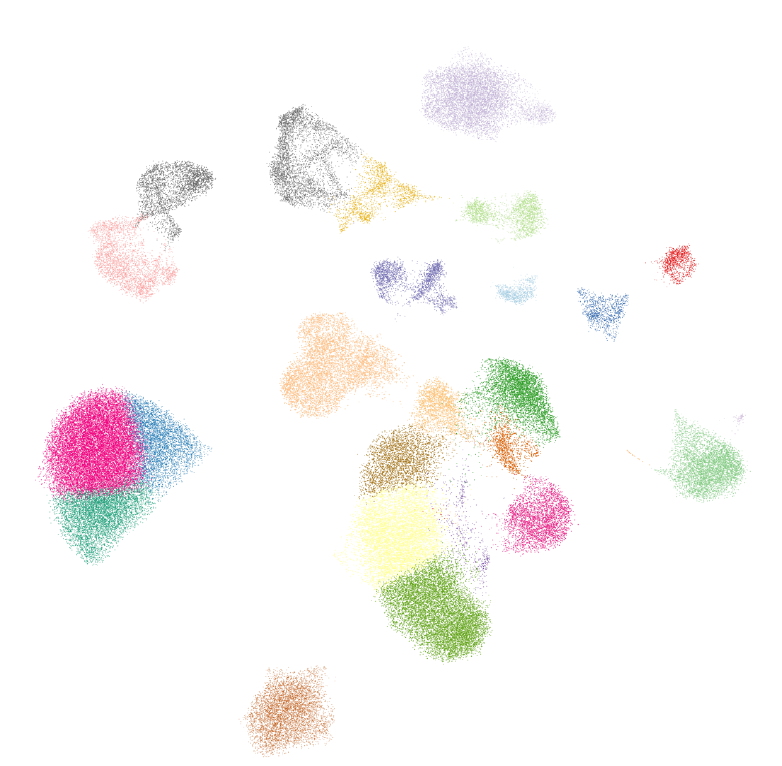
\includegraphics[width=\textwidth]{../paper/extended_plots/cell_proj_with_leiden.png}        
        \end{subfigure}
        \hspace{0.5cm}  
        \begin{subfigure}[t]{.45\textwidth}
            \caption{}
            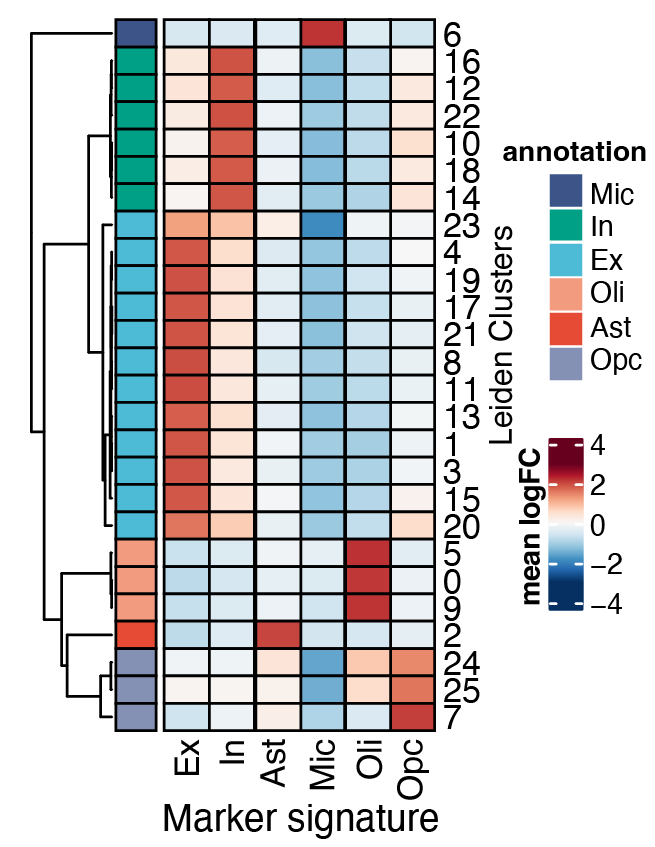
\includegraphics[width=\textwidth]{../paper/extended_plots/leiden_heatmap.png}        
        \end{subfigure}   
        \begin{subfigure}[t]{.3\textwidth}
            \caption{}
            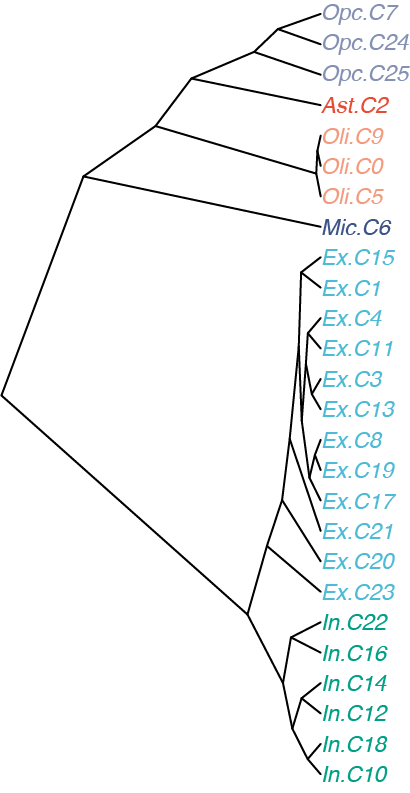
\includegraphics[width=\textwidth]{../paper/extended_plots/hierarchical_tree.png}        
        \end{subfigure}  
        \hspace{1cm}
        \begin{subfigure}[t]{.45\textwidth}
            \caption{}
            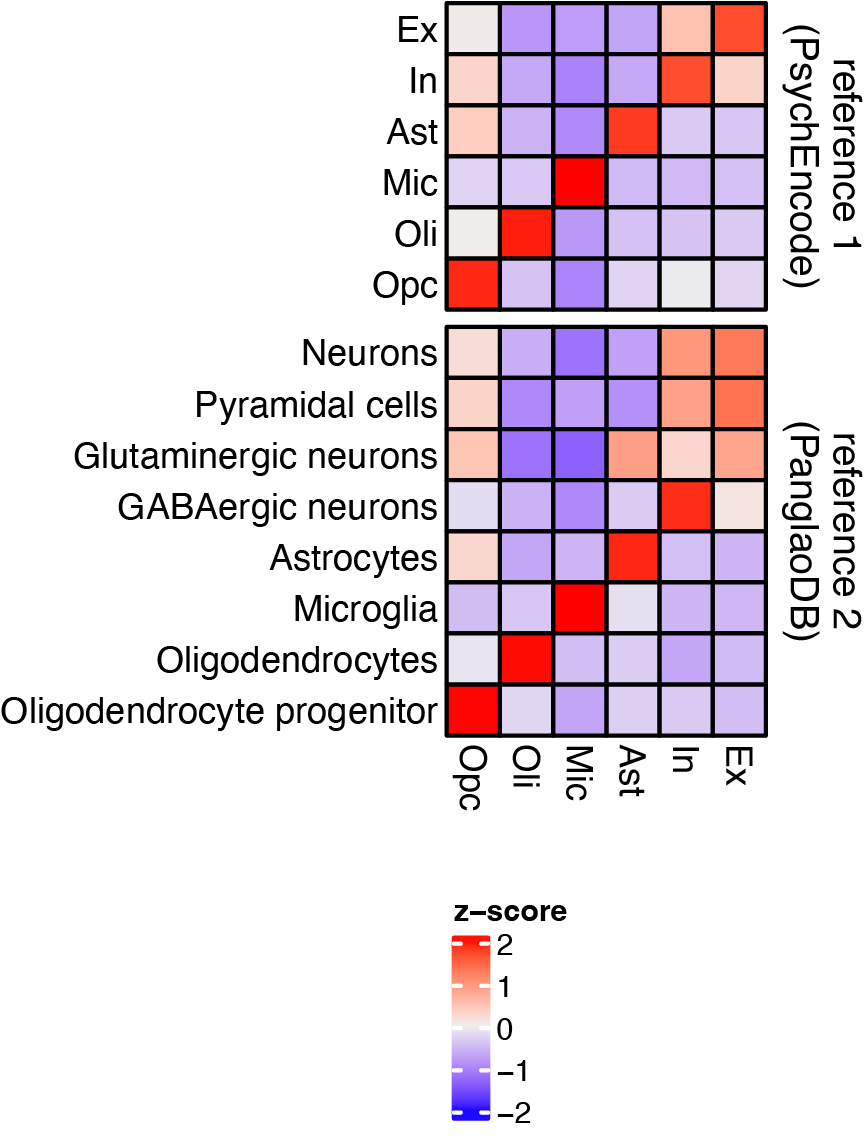
\includegraphics[width=\textwidth]{../paper/extended_plots/marker_hmap.png}        
        \end{subfigure}  
    \end{subfigure}
    \hspace{2cm}  
    \begin{subfigure}[t]{.25\textwidth}
        \caption{}
        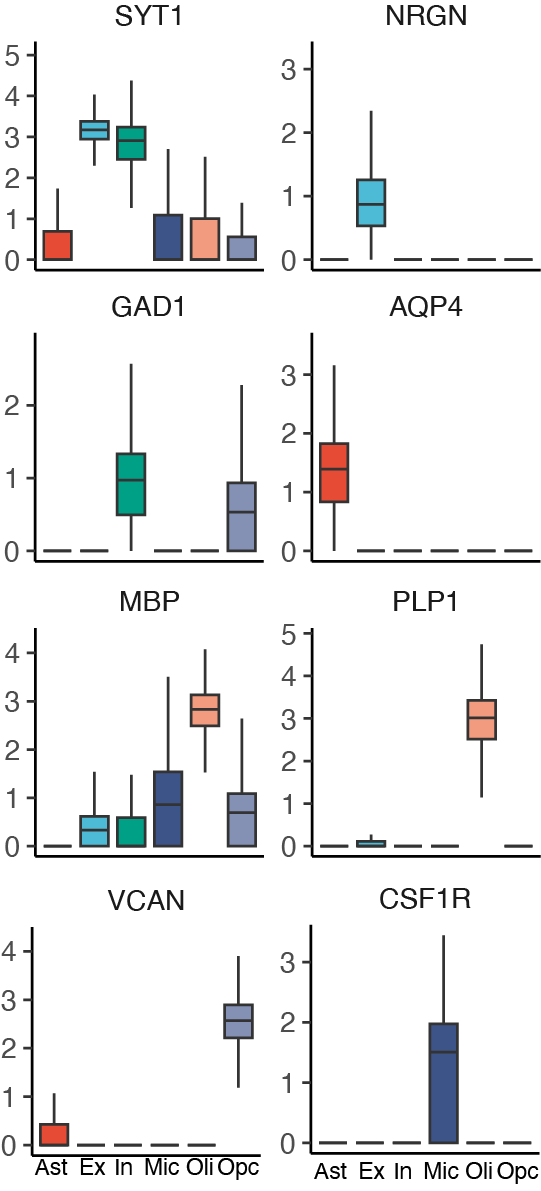
\includegraphics[width=\textwidth]{../paper/extended_plots/marker_boxplot.png}        
    \end{subfigure}    
    \par
    \begin{subfigure}[t]{.15\textwidth}
        \caption{}
        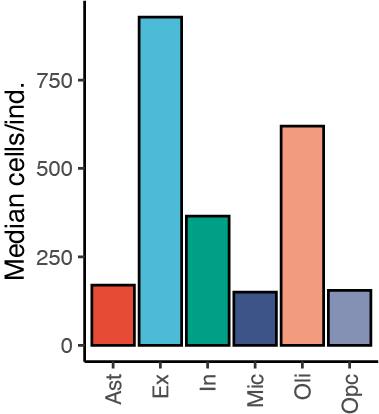
\includegraphics[width=\textwidth]{../paper/extended_plots/median_cells.png}        
    \end{subfigure} 
    \hspace{0.5cm}   
    \begin{subfigure}[t]{.25\textwidth}
        \caption{}
        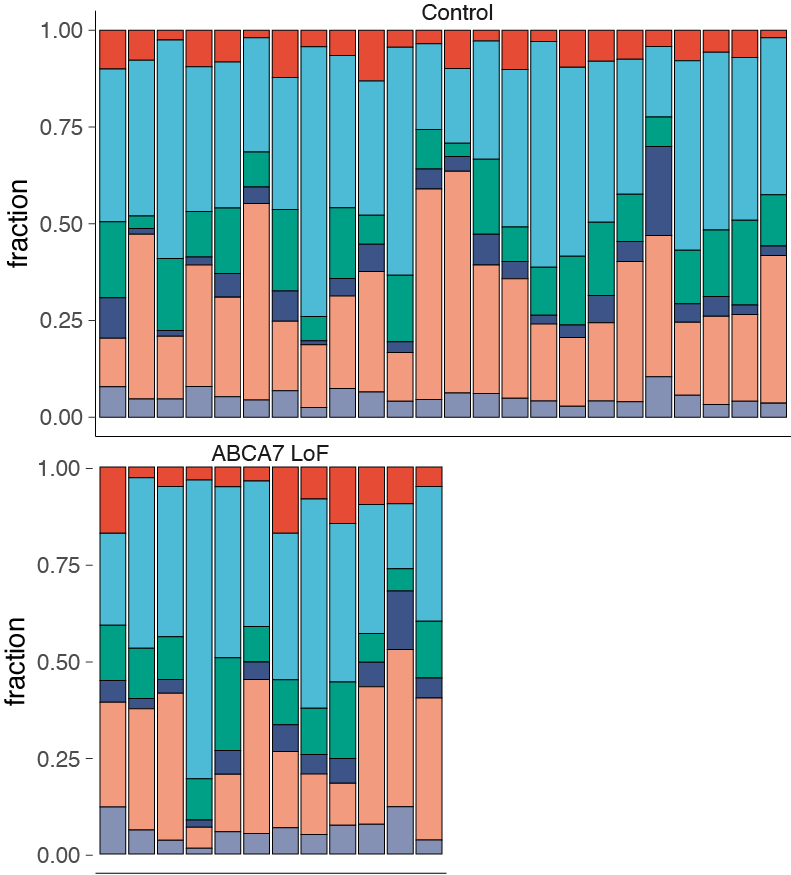
\includegraphics[width=\textwidth]{../paper/extended_plots/individual_fractions.png}        
    \end{subfigure}  
    \hspace{0.5cm}   
    \begin{subfigure}[t]{.25\textwidth}
        \caption{}
        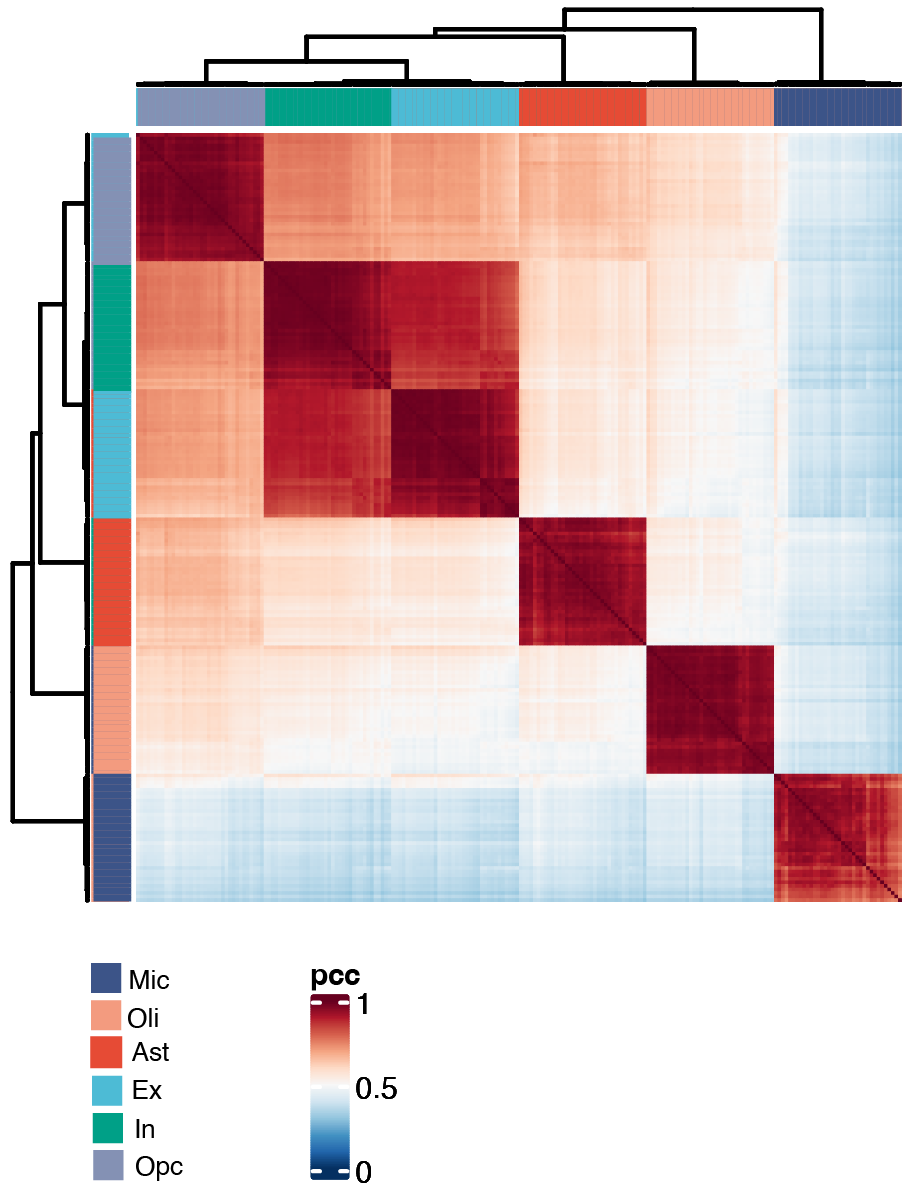
\includegraphics[width=\textwidth]{../paper/extended_plots/celltype_heatmap.png}        
    \end{subfigure}  
    \hspace{0.5cm}
    \begin{subfigure}[t]{.15\textwidth}
        \caption{}
        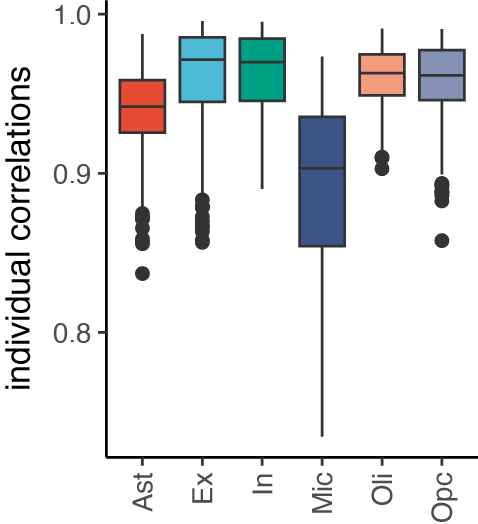
\includegraphics[width=\textwidth]{../paper/extended_plots/individual_correlations.png}        
    \end{subfigure}
\end{figure}

\textbf{Fig. S1: Overview of snRNA-sequencing Cell Type Annotations.}
\textbf{a,} Two-dimensional UMAP projections of individual cells from gene expression space, colored by Leiden clusters. 
\textbf{b,} Average marker gene expression (per-cluster mean log(fold-change)) for all marker genes for the cell type indicated along the x-axis. Log(fold-changes) are computed for the cluster of interest vs. all remaining clusters. Reference 1 (Table~\ref{tab:external_datasets}) marker genes were used. 
\textbf{c,} Cladogram visualizing subcluster relationships based on pairwise distances between per-cluster gene expression profiles. 
\textbf{d,} Average marker gene expression profiles (x-axis) per major cell type annotation (y-axis) for two marker gene references (Table~\ref{tab:external_datasets}). 
\textbf{e,} Per-cell distribution of select marker gene expression by cell type. Y-axis indicates log-counts. 
\textbf{f,} Median number of cells per cell type per individual. 
\textbf{g,} Cell type fraction by individual. 
\textbf{h,} Heatmap of individual-level gene expression correlations by cell type. 
\textbf{i,} Boxplot of individual-level gene expression correlations by cell type. 

